\documentclass{ximera}

\title{Assessment}

\newenvironment{objectives}{\begin{remark}\textbf{Objectives}\\}{\end{remark}}

\begin{document}
\begin{abstract}
\end{abstract}

\maketitle

\subsection{Assessment}
\begin{question}
What is the limit of the pictured function as $x$ approaches $5$? (You have 2 attempts.)

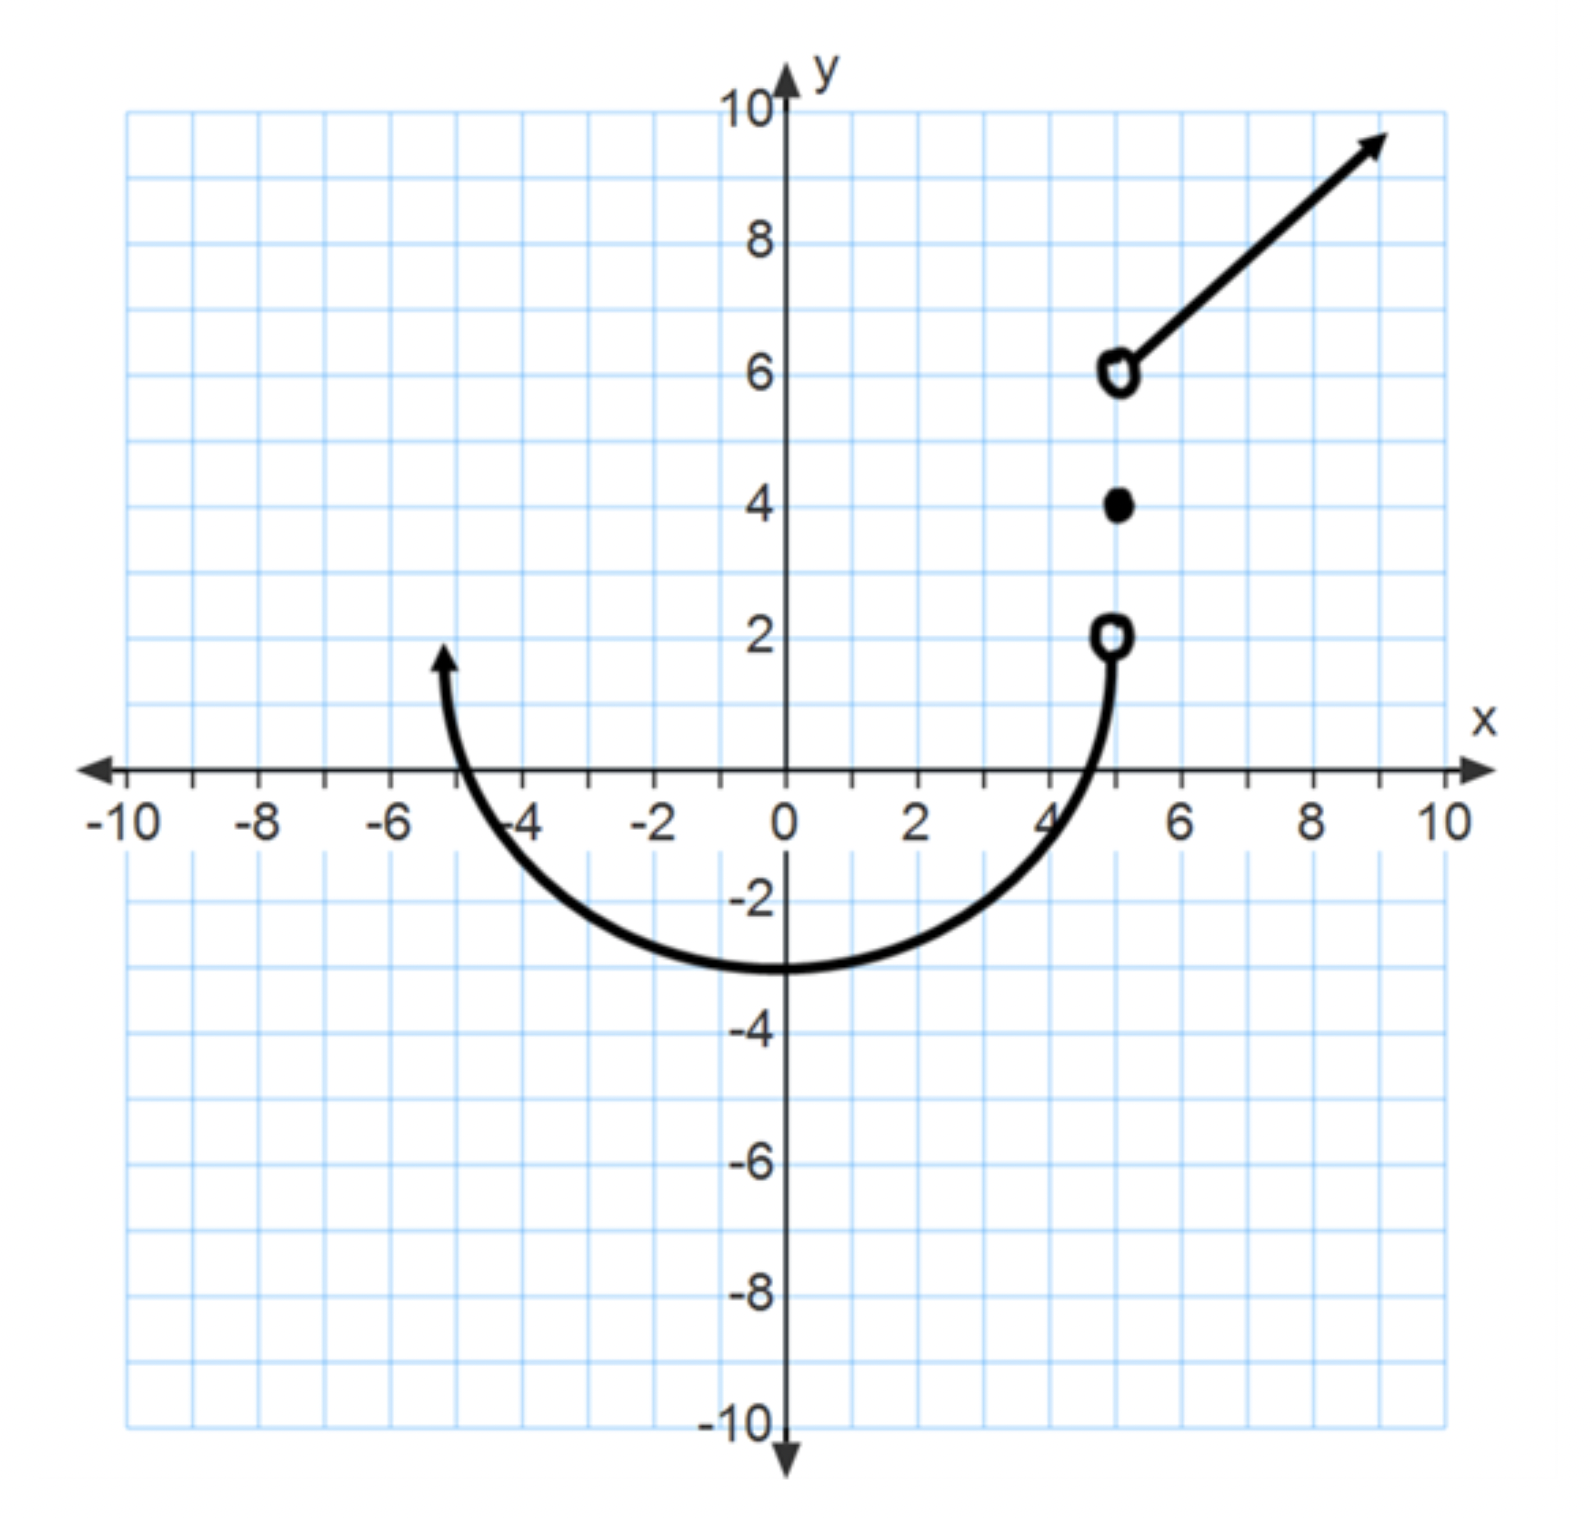
\includegraphics[width=0.5\textwidth]{graph3.png}
\begin{multipleChoice}  
\choice{4}
\choice[correct]{DNE}
\choice{2}  
\choice{6}
\end{multipleChoice}  

\begin{explanation}
    That's right! The correct response is DNE. While the one-sided limits do exist, the limit as $x \to 5$ of this function does not exist because the one-sided limits are not equal.
\end{explanation}
\end{question}

\end{document}